\documentclass[12pt,upcase]{umlthesis}
\usepackage{lipsum}
\usepackage{natbib}
\usepackage{graphicx}
\usepackage{float}

% use fancyhdr, to enable page style stuff (below)
\usepackage{fancyhdr}
\setlength{\headheight}{15.2pt}
\renewcommand{\headrulewidth}{0pt}

\pagestyle{plain}

\begin{document}
\title{Two-Fluid Collisional Magnetohydrodynamic Modeling}
\author{Qusai Al Shidi}
\prevdegrees{B.S., University of Toledo (2008)}
\department{Department of Physics and Applied Physics}
\degree{Doctor of Philosophy}
\degreemonth{May}
\degreeyear{2019}
\thesisdate{May 1, 2019}
\supervisor{Ofer Cohen}{Assistant Professor}
\maketitle

%%%%%%%%%%%%%%%%%%%%%%%%%%%%%%%%%%%%%%%%
\begin{abstract}
	Since the discovery of space plasmas, the space science community have been deriving fluid models of plasmas to best suit their scenarios. The simplest case is the ideal magnetohydrodynamic (MHD) model which assumes a collisionless perfectly-conducting plasma. Multi-fluid collisional MHD gives each fluid its own set of MHD equations while using collisions to set frictional and resistive terms between them. An important case of this nature is the solar chromosphere. The high density and relatively cold plasma ensures collision times are shorter than magnetic time scales. Multi-fluid collisional MHD has many cases from the Earth's ionosphere to stellar atmosphere and having a good grasp of the physics is important in studying these plasmas.
\end{abstract}

%%%%%%%%%%%%%%%%%%%%%%%%%%%%%%%%%%%%%%%%
\begin{acknowledgments}
An acknowledgments page is optional.
\end{acknowledgments}


%%%%%%%%%%%%%%%%%%%%%%%%%%%%%%%%%%%%%%%%
\tableofcontents
\listoffigures
\listoftables

\chapter{Introduction}

The word `plasma' was first used by \citet{Langmuir1928} to describe oscillations in a gaseous electron medium~\citep{Tonks1967}. It is a state of matter that is can be described as an ionized gas. It is the most common form of baryonic matter in the universe. We default to plasma descriptions of the medium between stars and planets. The sun is, for example, made mostly of ionized hot plasma. It is made of plasma and shoots out supersonic plasma called the solar wind. This plasma does not entirely contact the Earth due to shielding resulting from the Earth's magnetic field. Due to plasma's ionization, it has a tendency to travel on magnetic field lines. This does not mean the Earth is completely shielded from the solar wind. Many space weather events are due to solar plasma's effect on the Earth and its magnetic field. The sun is a very active star that has spontaneous flares, coronal mass ejections and active regions. Thus spontaneous storms occur on Earth and our understanding of the sun and space plasmas is essential to protect ourself against storms.

\section{The Sun}

Whenever we say `the sun' we do not mean any star---we mean \textit{our} star. The sun is a 4.6 billion year old yellow dwarf. It generates a lot of the energy we use for life on Earth. It creates this energy through nuclear fusion in its core, turning hydrogen into helium. The sun is mostly hydrogen with a small amount of helium and even smaller amounts of metal ions which require tremendous energy to fuse. The sun has six regions (from innermost to outermost): the core, the radiative zone, the covection zone, the photosphere, the chromosphere and the corona. The core is where the fusion happens. Here is where hydrogen is made into helium and other metals. The radiative zone and convection zone is where the energy travels radially upwards to wards the surface, the photosphere. The photosphere is the surface of the Sun. Here photons are trapped but the ones that do escape mimic black-body radiation (not perfectly). It is optically thick and is the white light we see when looking at the Sun. Above the photosphere is the atmospheric layer, the chromosphere, which we will go in much detail about in this dissertation. Above that, is the corona which is what gives the sun its tendrils and the hair we give our cartoon drawings of the sun.

\subsection{The Chromosphere}

The chromosphere is the interface between the surface, the photosphere, and the outer atmosphere, the corona. The plasma in it is partially ionized which means it consists of two kinds of plasma: ionized (charged) plasma, and neutral (uncharged) plasma. This means the charged plasma is affected by Lorentz forces while the uncharged plasma is not. This is a result of the temperature of the chromosphere and the composition of the plasma convected in the convection zone. The plasma has a high temperature in Earth standards but to the sun it is relatively cold. The temperature of the corona, which keep in mind is the outermost layer, is in the million of degrees in Kelvin. While most of the chromosphere and the photosphere is 5000K-6500K. This discrepancy in the temperature of the lower layers to the higher layers is called the coronal heating problem. The coronal heating problem is an outstanding problem in physics which makes understanding the chromosphere of special importance. Why is the corona hotter than the chromosphere?

\begin{figure}[ht!]\label{fig:chromoprofile}
	\centering
	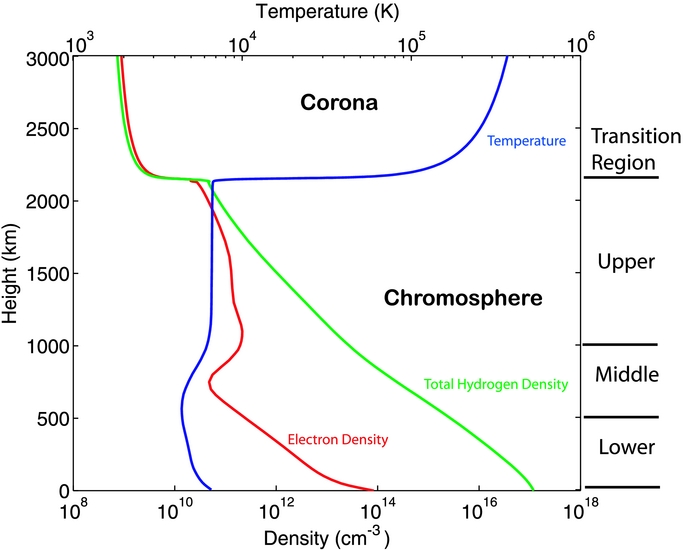
\includegraphics[width=0.75\linewidth]{chromoprofile.jpg}
	\caption{A view of the upper, middle and lower chromosphere. The chromosphere is partially ionized and is much colder than the corona (above the transition region).~\citep{Song2014}}
\end{figure}

%%%%%%%%%%%%%%%%%%%%%%%%%%%%%%%%%%%%%%%%
%%%%%%%%%%%%%%%%%%%%%%%%%%%%%%%%%%%%%%%%
\chapter{Examples}
This chapter will show as much of the document class\footnote{This is a short footnote.} as possible. The footnotes\footnote{You'll find that this footnote is overly verbose and won't fit on a single line. If I have written the document class correctly, then the indentation will match the specification in the UML Thesis Guide.} are required to be indented in a particular way, for example.

\begin{quote}
  This is a paragraph quoted from somewhere else. It must be single-spaced and indented on both sides.
\end{quote}

In Table~\ref{tab:fruits} you can see what a table will look like. Refer to Figure~\ref{fig:square} to see a figure.

\begin{table}[h]\label{tab:fruits}
  \centering
  \caption[Comparison of fruits]{Only fruits of the same type may be compared safely.}
  \begin{tabular}{l|cc}
    & Apples & Oranges \\
    \hline
    Apples & yes & no \\
    Oranges & no & yes \\
  \end{tabular}
\end{table}

\lipsum[1]

\begin{figure}\label{fig:square}
  \centering
  \rule{2in}{2in}
  \caption{A black square.}
\end{figure}

\section{A Section}
This is what a main section heading looks like.

\lipsum[1]

\subsection{A Subsection}
Sub sections look like this.

\lipsum[1]

\subsubsection{A Sub-subsection (Don't go this deep!)}
Don't use sub-subsections.

\lipsum[1]

\section{Another Section}
This proves that the section numbering works.

%%%%%%%%%%%%%%%%%%%%%%%%%%%%%%%%%%%%%%%%
\chapter{Requirements}

\newcommand{\pkg}[1]{\textsf{#1}}

This document class requires \pkg{natbib},  \pkg{setspace}, and \pkg{tocloft}, which are probably already a part of your \LaTeX\ distribution.

%%%%%%%%%%%%%%%%%%%%%%%%%%%%%%%%%%%%%%%%
%\nocite{*}
\bibliographystyle{plainnat}
\bibliography{phd-thesis}

%%%%%%%%%%%%%%%%%%%%%%%%%%%%%%%%%%%%%%%%
\appendix
\chapter{Appendix Chapter}
\lipsum[2]

\end{document}
